\pegasus{}~\cite{Vogt:2004ns} is a Fortran program aimed for \pdf{} evolution.
The program solves \dglap{} numerically in $N$-space up to \nnlo{}.
\pegasus{} can only deal with \pdfs given as a fixed functional form and is
not interfaced with \lhapdf{}.

As shown in \cref{fig:eko/LHAbench}, the agreement of \eko{} with this tool is better than with \apfel{},
especially for valence-like quantities, for which an exact solution is possible, where we reach
$\mathcal{O}(10^{-6})$ relative accuracy.
This is expected and can be traced back to the same \dglap{} solution strategy in Mellin space.

Similarly to the \apfel{} benchmark, we assert that the precision of our benchmark with \pegasus{} is not affected
by the different \qcd{} perturbative orders, as visible in \cref{fig:eko/Pegasusbench_pto}.
As both, \apfel{} and \pegasus{}, have been benchmarked against
\hoppet{}~\cite{Salam:2008qg} and \qcdnum{}~\cite{Botje:2010ay} we conclude
to agree also with these programs.

\begin{figure}
    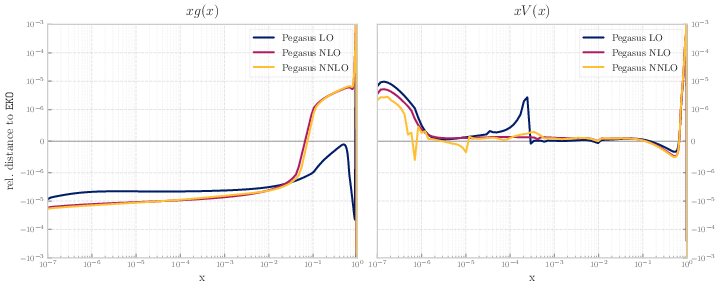
\includegraphics[width=\linewidth]{ch-eko/Pegasus_bench_pto.png}
    \caption{Same of \cref{fig:eko/Apfelbench_pto}, now comparing to \pegasus{}~\cite{Vogt:2004ns}.
        \label{fig:eko/Pegasusbench_pto} }
\end{figure}
